\documentclass{report}
\usepackage{graphicx}
\usepackage{xcolor}
\usepackage[a4paper, total={6in, 8in}]{geometry}
\usepackage{color}
\usepackage{multicol}
\setlength{\columnseprule}{1pt}
\def\columnseprulecolor{\color{blue}}

\graphicspath{ {./image/} }

\title{Babar Forecasting}
\date{2020}

\begin{document}
\maketitle

\chapter{Goal}

\section{The Problem}

\section{Our Solution}

\chapter{Data Management}

\section{Selection and Gathering Sales Data}

There are too many products to have a prediction for each one. So we decided to gather them into categories. We want to gather them into pertinent groups so that the forecast can really help the bar.

\subsection{First Selection}

The first step is to choose which product we are going to take account of. We choosed to focus our work on the drinks sales that had at least been sold ???. So we exclude any food or other kind of sales.

SQL Request too extract those product : \\
 \\

CREATE TABLE WantedProducts AS
    SELECT babar$\_$server$\_$purchase.* FROM babar$\_$server$\_$purchase JOIN babar$\_$server$\_$product ON product$\_$id = babar$\_$server$\_$product.id WHERE NAME = 'Leffe' OR NAME = 'Hoegaaden blanche' OR NAME = 'Desperados' OR NAME = 'Smirnoff' OR NAME = 'Pastis' OR NAME = 'Hard' OR NAME = 'Grimbergen' OR NAME = 'Chimay Rouge' OR NAME = 'Chimay Bleue' OR NAME = 'Kro Demi' OR NAME = 'Cidre Demi' OR NAME = 'Pelforth' OR NAME = 'Kwak' OR NAME = 'Kir' OR NAME = 'Kro Pinte' OR NAME = 'Cidre Pinte' OR NAME = 'Cocktail Hard' OR NAME = 'Chimay Blanche' OR NAME = 'Shot'  OR NAME = 'Blanche Demi' OR NAME = 'Blanche Pinte' OR NAME = 'Cidre Doux/Brut' OR NAME = 'Ambree demi' OR NAME = 'Ambree Pinte'  OR NAME = 'Delirium' OR NAME = 'Rouge Pinte' OR NAME = 'Sangria' OR NAME = 'Karmeliet Triple' OR NAME = 'Duvel' OR NAME = 'Granita Hard' OR NAME = 'Skoll' OR NAME = 'Rouge Demi' OR NAME = '$1664$ Blanche' OR NAME = 'Chimay bleue' OR NAME = 'Pecheresse' OR NAME ='Cuvee des Trolls'  OR NAME = 'Kriek' OR NAME = 'Elephant Pinte' OR NAME = 'Elephant Demi' OR NAME = 'Maredsous Triple' OR NAME = 'Hard Qualite' OR NAME = 'BrewDog Punk IPA' OR NAME = 'JagerBomb' OR NAME = 'Cubanisto' OR NAME = 'Chouffe Pinte' OR NAME = 'Chouffe Demi' OR NAME = 'Corona' OR NAME = 'Tigre Bock' OR NAME = 'Troll Pinte' OR NAME = 'Troll Demi' OR NAME = 'Triple Karmeliet Pinte' OR NAME = 'Triple Karmeliet Demi' OR NAME = 'Paix Dieu $33$cL' OR NAME = 'Grim Triple Demi' OR NAME = 'Grim Triple Pinte' OR NAME = 'Cherry chouffe' OR NAME = 'Delirium rouge pinte' OR NAME = 'bush ambree' OR NAME = 'San Miguel';

List of considered product :

So now we have a data table gathering only the product we choose.

\subsection{Other products that could be considered}

\subsection{Regrouping them into categories}

A majority of this product has been coming and leaving from the bar menu so their sales aren't usable one by one. Therefor we decided to group them into pertinent categories. But how to choose this categories ? Here are our first thought.

\begin{multicols}{2}
\textbf{High Degree Beers}
\begin{itemize}
\item Chimay Bleu
\item Kwak
\item Karmeliet Triple
\item Duvel
\item Chimay bleue
\item Maredsous Triple
\item Chouffe Pinte
\item Chouffe Demi
\item Triple Karmeliet Pinte
\item Triple Karmeliet Demi
\item Grim Triple Pinte
\item Grim Triple Demi
\item bush ambree
\item Delirium
\item Elephant Pinte
\item Elephant Demi
\end{itemize}

\columnbreak

\textbf{Normal Degree Beers}
\begin{itemize}
\item Leffe
\item Grimbergen
\item Kro Demi
\item Kro Pinte
\item Pelforth
\item Skoll
\item BrewDog Punk IPA
\item Tigre Bock
\item Troll Pinte
\item Troll Demi
\item Cuvée des trolls
\item Paix Dieu 33cL
\item San Miguel
\item Ambrée Pinte
\item Ambrée Demi
\end{itemize}

\end{multicols}

\pagebreak

\begin{multicols}{3}

\textbf{Not Beer}
\begin{itemize}
\item Smirnoff
\item Pastis
\item Hard
\item Kir
\item Cocktail Hard
\item Shot
\item Rouge Pinte
\item Rouge Demi
\item Sangria
\item Granita Hard
\item Hard Qualite
\item JagerBomb
\end{itemize}

\columnbreak

\textbf{Special Beers}
\begin{itemize}
\item Desperados
\item Cidre Demi
\item Cidre Pinte
\item Cidre Doux/Brut
\item Cubanisto
\item Corona
\end{itemize}

\columnbreak

\textbf{Aromatized Beer}
\begin{itemize}
\item Chimay Rouge
\item Hoegaaden blance
\item Chimay Blanche
\item Blanche Demi
\item Blanche Pinte
\item 1664 Blanche
\item Pecheresse
\item Kriek
\item Cherry chouffe
\item Delirium rouge pinte
\end{itemize}

\end{multicols}


Other idea : Aromatize beer and Special together

Those are ideas of the categories, at every time at least one product of each category was being sold, assuring the continuity of sales in each categories. The goal is having sales that are homogene on a year scale.


\subsection{SQL code for product gathering}

DROP TABLE IF EXISTS `High$\_$Degree$\_$Beer`;

CREATE TABLE `High$\_$Degree$\_$Beer`
	AS SELECT babar$\_$server$\_$purchase.* FROM babar$\_$server$\_$purchase JOIN babar$\_$server$\_$product ON babar$\_$server$\_$purchase.product$\_$id = babar$\_$server$\_$product.id WHERE
	NAME = 'Chimay Bleue' OR NAME = 'Chimay Bleu' OR NAME = 'Kwak' OR NAME = 'Karmeliet Triple' OR NAME= 'Duvel' OR NAME = 'Maredsous Triple'
	OR NAME = 'Chouffe Pinte' OR NAME = 'Chouffe Demi'  OR NAME = 'Triple Karmeliet Pinte' OR NAME = 'Triple Karmeliet Demi'  OR NAME = 'Grim Triple Pinte'
	OR NAME = 'Grim Triple Demi' OR NAME = 'bush ambrée' OR NAME = 'Delirium' OR NAME = 'Elephant Pinte' OR NAME = 'Elephant Demi';



DROP TABLE IF EXISTS `Normal$\_$Degree$\_$Beer`;

CREATE TABLE `High$\_$Degree$\_$Beer`
	AS SELECT babar$\_$server$\_$purchase.* FROM babar$\_$server$\_$purchase JOIN babar$\_$server$\_$product ON babar$\_$server$\_$purchase.product$\_$id = babar$\_$server$\_$product.id WHERE
	NAME = 'Leffe' OR NAME = 'Grimbergen' OR NAME = 'Kro Demi' OR NAME = 'Kro Pinte' OR NAME = 'Pelforth' OR NAME = 'Skoll' OR NAME = 'BrewDog Punk IPA'
	OR NAME = 'Tigre Bock' OR NAME = 'Troll Pinte' OR NAME = 'Troll Demi' OR NAME ='Cuvée des trolls' OR NAME = 'Paix Dieu 33cL' OR NAME = 'San Miguel'
	OR NAME = 'Ambrée pinte' OR NAME = 'Ambrée demi';



DROP TABLE IF EXISTS `Not$\_$Beer`;

CREATE TABLE `High$\_$Degree$\_$Beer`
	AS SELECT babar$\_$server$\_$purchase.* FROM babar$\_$server$\_$purchase JOIN babar$\_$server$\_$product ON babar$\_$server$\_$purchase.product$\_$id = babar$\_$server$\_$product.id WHERE
	NAME = 'Smirnoff' OR NAME = 'Pastis' OR NAME = 'Hard' OR NAME = 'Kir' OR NAME = 'Cocktail Hard' OR NAME = 'Shot' OR NAME = 'Rouge Pinte' OR NAME = 'Rouge Demi'
	OR NAME = 'Sangria' OR NAME = 'Granita Hard' OR NAME = 'Hard Qualité' OR NAME  = 'JagerBomb';


\section{Time Scale}

We think that a Weekly prediction can be done, so we'll consider the sales week by week (Time series approach). If we have difficulties doing it we will consider doing it monthly but then the forecast would be much less usable. (Time series approach)

We will also maybe consider a year index. Indeed promotion aren't all the sames therefor they don't consume the same quantities. Adding a bias for each promotion (which would be compute thanks to the first month of data ? september ?) could maybe increase the accuracy of our estimations.\\
When to start ? Beginning of 2011 or rentree 2011 ?

\subsection{Sorting By week}

For each week we will sum the sales for each categories. The weeks will be register by a index of week from 1 to 52, and a year. So 2 keys.

I don't think that I can sort the data by week by using SQL, so I'll do a python code that do that. The results will be a table with the sales for each category for each week.


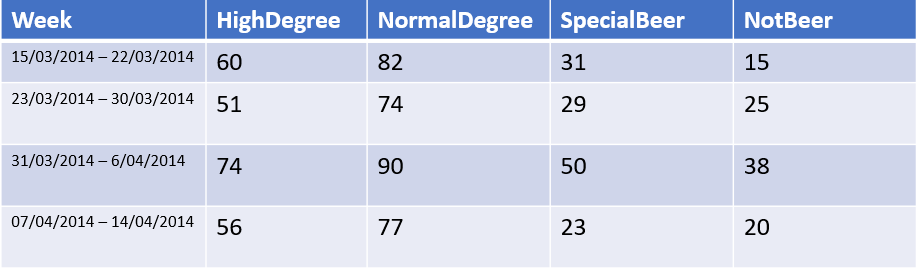
\includegraphics[scale = 0.8]{FormatTable}

\section{Other used Data}

In order to do our prediction we thing about using the following features :
\begin{itemize}
\item Day before next holiday
\item Day before next exam
\item Day after exam or holiday ?
\item Day before next large event ?
\end{itemize}

We think that those are the main influences on whether people buy more or less drinks in a bar.

\subsection{Holidays}

The holidays data is gather in a CSV file with 3 columns, Year, WeekNo and Holiday. If the week is a Holiday week then the holiday column contains a 1. If it's a work week then there is a 0. After thinking about it we decided to not only consider if the week is or isn't a holidays week but also count the number of week before the next holidays. Indeed we forsee that people tend to buy more in a Bar when a Holiday is near.
So the data given to the machine learning model will be the counter to the next holiday.

\subsection{Exams}

The Exams data is also gathered in a CSV file with 3 columns, Year, WeekNo and Exam. If there is a Exam this week the Exam column contains a 1 and a 0 if not. As we did for the holidays what would interest us is a counter to the next exam. But in the case of exams we also want to transcript the possibility of several week of exams following each other. So our idea is to examine the 3 following weeks and ponderate them (the first is more impactfull than the third one, with coefficient 3,2,1).


! HOWEVER ! : We think about being more precise and adding a value '2' that will transcript the importance of some exams.

\subsection{Promotion}


Adding a coefficient considering the promotion ! Every promotion doesn't drink the same, a coefficient should be schoolyear based. SO we just add a feature indicating the "promotion". We hope that the ML model will be able to consider the feature and balance the sales data of each year.


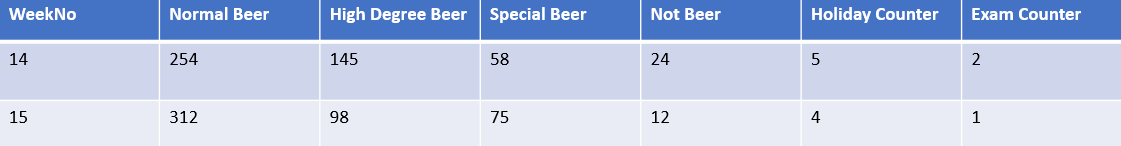
\includegraphics[scale=0.7]{DataModel}
\chapter{Model Selection}

Now the core of our work is to choose the best method to predict from our data. Or goal is to look in the dataset for features such as trends, cyclical fluctuations, seasonality, and behavioral patterns.


Here are the algorithm that we read about and could be used to forecast sales :
\begin{itemize}
\item KNN Regressor
\item Random Forest
\item Neural network
\end{itemize}

\section{KNN Regressor}

The KNN algorithm uses ‘feature similarity’ to predict the values of any new data points. This means that the new point is assigned a value based on how closely it resembles the points in the training set.


\section{Random Forest}

The Decision Tree algorithm has a major disadvantage in that it causes over-fitting.
This problem can be limited by implementing the Random Forest Regression in place of the Decision Tree Regression. Additionally, the Random Forest algorithm is also very fast and robust than other regression models.
To summarize in short, The Random Forest Algorithm merges the output of multiple Decision Trees to generate the final output.

\section{Neural Network}




See Regularization ? ML course 24 november.


\subsection{Promotion}
Another important feature is the school year !

\chapter{Finding the best Forecasting Method}



\section{Comparing Models}

In order to compare models we need to choose a metric. 

\subsection{Choosing a Metric}

There are the three possible metric that we consider : score ($R^2$) / Absolute Error / Squared Error.
We think that the best metric to use is the mean squared error (RMSE), but in a concrete way the best one is actually the absolute error that is the most indicative as it shows the actual difference that the bar will encounter.


\subsection{Choosing a model}


Difference between shuffle and not shuffle is very notable ! So our model is missing something that considerate the year maybe ? We thought adding the promotion as a feature would be a solution but apparently that's not enough




\section{Comparing the importance of features}

In order to see the importance of features we are going to try different combination of them.

\begin{itemize}
\item Promotion : It seems to be a very important feature, when we take it out the results drops 
\item Exams : It doesn't affect the results as much as promotion but it still taking them up, when dropping this feature we observe a small drop in the results
\item Week Number : Very important, as promotion dropping it really worsen our results
\item Week to holiday : Like exam
\end{itemize}

Ok it is maybe because we invented most of the exmas and week to holiday ! We need to find the real ones !

\chapter{Development Ideas}

Adding a coefficient considering the promotion ! Every promotion doesn't drink the same, a coefficient should be schoolyear based.






\chapter{Inspirations}

https://towardsdatascience.com/sales-forecasting-from-time-series-to-deep-learning-5d115514bfac : Forecasting principles and basis

https://medium.com/analytics-vidhya/walmart-sales-forecasting-d6bd537e4904 : Forecasting at Walmart







\end{document}
